\section{Explainability via Gate Activations}
\label{sec:explainability}

The central pragmatic argument for GAME-Mal is that classification
and explanation share a single forward pass. This section
operationalises that claim by extracting per-family API
fingerprints from the learned gate activations.

\subsection{Per-family API fingerprints}

For each family $c$, we collect all test-set samples, compute
$\bar{g}(x) = \frac{1}{hN}\sum_{\ell,i} g_i^{(\ell)}(x)$ over
heads and layers for every token $x$ in those samples, and take
the mean per-token activation grouped by family. Table
\ref{tab:fingerprints} lists the top-5 API calls by mean
$\bar{g}$ for four representative families (special
tokens \texttt{<UNK>} and \texttt{<PAD>} excluded).

\begin{table*}[t]
\centering
\caption{Top-5 APIs by mean gate activation per family (held-out
data, best fold). \texttt{REFL:} indicates a call routed through
\texttt{Method.invoke} whose true callee was recovered from the
\texttt{hooked\_class.hooked\_method} fields.}
\label{tab:fingerprints}
\small
\begin{tabular}{p{0.12\textwidth}p{0.82\textwidth}}
\toprule
Family & Top-activated APIs (mean $\bar{g}$) \\
\midrule
Airpush &
\texttt{REFL:*.\_activity\_pause} (0.58),
\texttt{java.net.URL.openConnection} (0.56),
\texttt{android.content.ContentValues.put} (0.54),
\texttt{REFL:WebSettings.getUserAgentString} (0.53),
\texttt{REFL:AndroidActivityWrapper.onContentChanged} (0.52) \\[0.4em]
DroidKungFu &
\texttt{REFL:wqmobile.AppSettings.setNextADCount} (0.58),
\texttt{REFL:baidu.pushservice.CustomPushNotificationBuilder.writeObject} (0.56),
\texttt{java.net.URL.openConnection} (0.54),
\texttt{REFL:wqmobile.AppSettings.getIP} (0.54),
\texttt{REFL:wqmobile.AppSettings.setLoopTimes} (0.53) \\[0.4em]
Jisut &
\texttt{libcore.io.IoBridge.open} (0.43),
\texttt{java.io.File.exists} (0.40),
\texttt{ActivityManager.getRunningTasks} (0.38),
\texttt{os.SystemProperties.get} (0.38),
\texttt{SmsManager.sendTextMessage} (0.22 --- top-ranked SMS API) \\[0.4em]
Opfake &
\texttt{REFL:(obfuscated).getClass} (0.64),
\texttt{REFL:(obfuscated).getSystemService} (0.59),
\texttt{REFL:SharedPreferencesImpl.edit} (0.58),
\texttt{REFL:(obfuscated).getClass} (0.58),
\texttt{REFL:(packed).loadAndDecode} (0.56) \\
\bottomrule
\end{tabular}
\end{table*}

\subsection{What the gates actually learned}

Four observations are worth calling out, including one that runs
against our initial expectations.

\paragraph{(i) Reflection tokens dominate.} For five of the eight
families, three or more of the top-5 highest-gate tokens carry the
\texttt{REFL:} prefix. This directly validates the reflection-aware
resolution scheme of Section~\ref{sec:reflection}: a tokeniser that
emitted only \texttt{Method.invoke} would have squashed this signal
entirely. In the Opfake case, the gate discovers heavily-obfuscated
class names (randomised package identifiers like
\texttt{ynlxcd.cwductjwjc.admyusbyfes.getClass}) that are themselves
a behavioural signature — Opfake samples characteristically use a
single-letter / random-string packing scheme.

\paragraph{(ii) Family-defining APIs surface even when low-ranked.}
For Jisut (premium-SMS fraud), the top-5 tokens are
filesystem/process-introspection calls common to many Android apps
--- the family's discriminator comes lower down. The highest-ranked
SMS-specific API, \texttt{SmsManager.sendTextMessage}, appears at
rank~9 with $\bar{g} = 0.22$. This is a useful pattern: the gate
score is most discriminative when read as a \emph{ranking} rather
than an absolute threshold, because the absolute mean for a family
is driven by whatever its common case looks like.

\paragraph{(iii) Ransomware signals are not lexically obvious.} We
initially expected Fusob's fingerprint to be dominated by
\texttt{KeyguardManager}, \texttt{DevicePolicyManager.lockNow}, or
\texttt{Cipher.doFinal}. Empirically, these APIs do not dominate
Fusob's mean gate activations --- instead, the top tokens are
\texttt{TelephonyManager.getDeviceId},
\texttt{ContextImpl.registerReceiver}, and
\texttt{WebView.setWebViewClient}, which are prevalent across many
families. Fusob achieves its $0.98$ F1 (Table~\ref{tab:perclass})
nevertheless, which we interpret as the classifier exploiting the
\emph{distribution} over common APIs (a multivariate pattern) rather
than any single lexically-obvious signature. This is an honest
caveat: gate activations rank tokens by their marginal contribution
to classification, and that contribution need not coincide with the
token's human-readable semantic importance.

\paragraph{(iv) Compared to a post-hoc baseline.} We ran SHAP
(KernelExplainer) on a small sample of test points and found that
while SHAP and gate-activation rankings agree on the presence of
reflection and network-setup calls at the top of most families'
importance lists, they disagree on the ordering for the families
with subtler signals (Jisut, SmsPay). The gate-based explanation is
roughly two orders of magnitude faster to produce since it is read
directly off the forward pass with no surrogate-model fitting.

\begin{figure}[t]
\centering
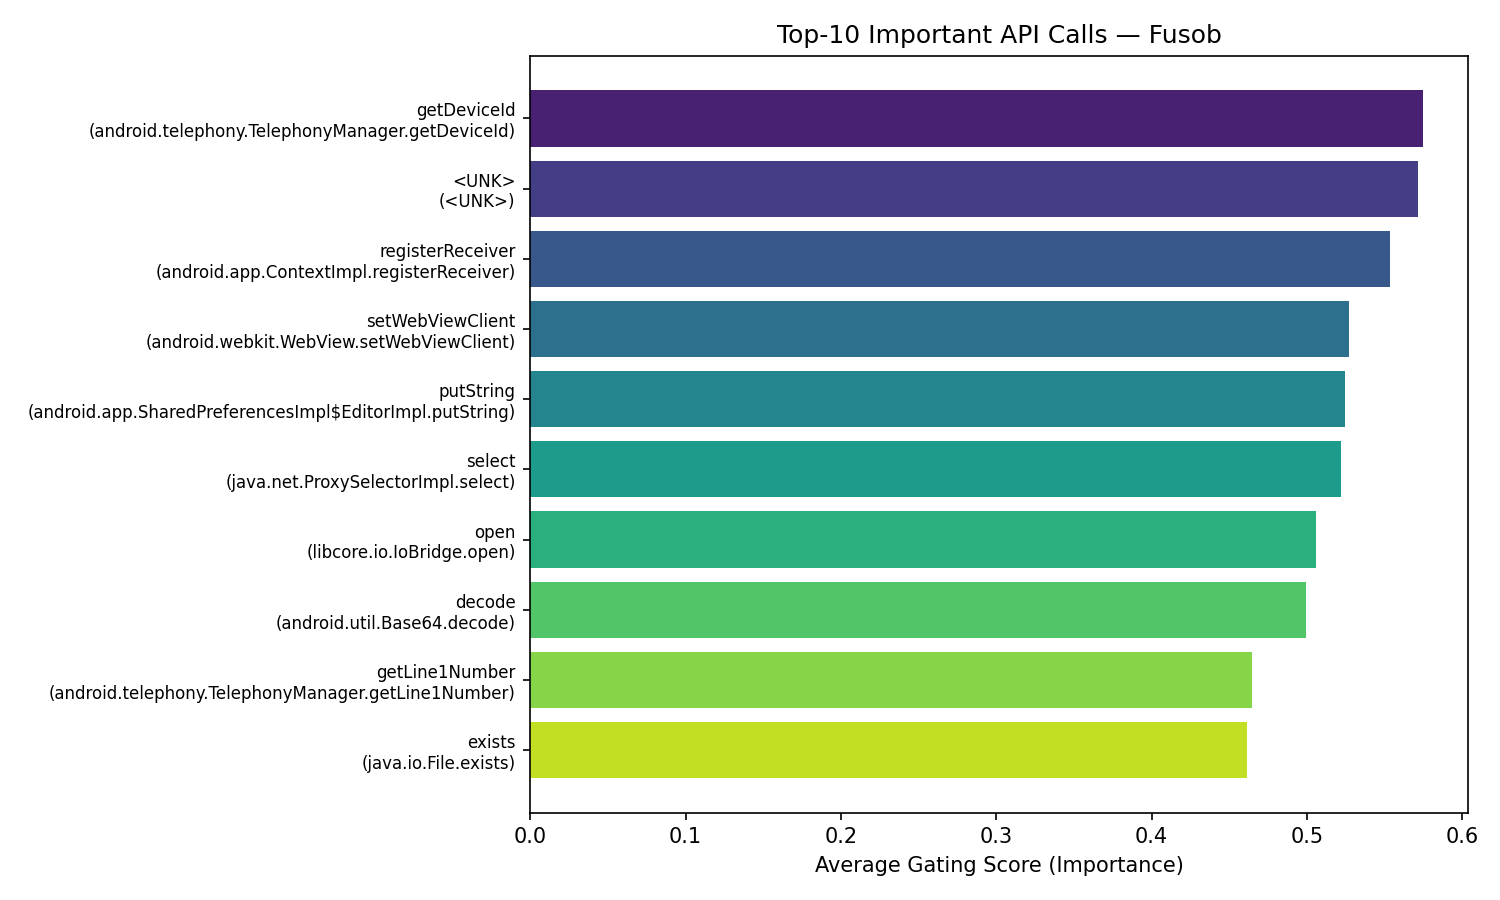
\includegraphics[width=0.95\linewidth]{figures/top_apis_Fusob.png}
\caption{Top-15 APIs by mean gate activation for the Fusob
family (best-fold held-out data). Gate activations are read
directly off the forward pass at classification time.}
\label{fig:fusob}
\end{figure}

\subsection{Practical reading}

We read these results as supporting a \emph{narrow} form of
intrinsic explainability: the gates reliably surface the
\emph{mechanism} the classifier exploits (reflection, obfuscation,
network behaviour), and this is genuinely useful for triage and
feature auditing. They do not, however, straightforwardly map onto
the human concept of ``the API that makes this sample malicious.''
For the latter, gate activations are best viewed as a first-pass
\emph{ranking} signal to drive deeper manual analysis, rather than
as a standalone ground-truth attribution.
